\usetikzlibrary{positioning}

\begin{tikzpicture}

	\coordinate (ref) at (0, 0);

	\node[below = 0.1 of ref] (nn) {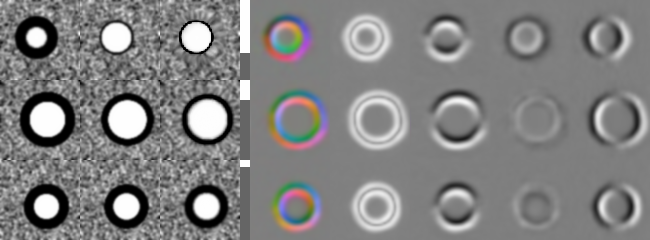
\includegraphics[width=\textwidth]{noise_sparse}};

	\node[above right = 0.05 and 0.7 of nn.north west] (x) {$x\vphantom{\norm{v}_2}$};
	\node[right = 1.6 of x.west] (y)	{$y\vphantom{\norm{v}_2}$};
	\node[right = 1.6 of y.west] (yhat)	{$\hat y\vphantom{\norm{v}_2}$};
	\node[right = 0.9 of yhat.west] (t)	{$t\vphantom{\norm{v}_2}$};
	\node[right = 0.9 of t.west] (v)	{$v\vphantom{\norm{v}_2}$};
	\node[right = 1.4 of v.west] (mag)	{$\norm{v}_2$};
	\node[right = 1.8 of mag.west] (vx)	{$v_x\vphantom{\norm{v}_2}$};
	\node[right = 1.6 of vx.west] (vy)	{$v_y\vphantom{\norm{v}_2}$};
	\node[right = 1.6 of vy.west] (vz)	{$v_z\vphantom{\norm{v}_2}$};


\end{tikzpicture}
